\documentclass[conf]{new-aiaa}
%\documentclass[journal]{new-aiaa} for journal papers
\usepackage[utf8]{inputenc}

\usepackage{graphicx}
\usepackage{amsmath}
\usepackage[version=4]{mhchem}
\usepackage{siunitx}
\usepackage{longtable,tabularx}
\setlength\LTleft{0pt} 

\title{Fly-Back of a Scramjet-Powered Accelerator}

 \author{
 	Sholto O. Forbes-Spyratos%
 	\footnote{Ph.D. Candidate, Centre for Hypersonics, School of Mechanical and Mining Engineering. Member AIAA.}
 	\ ,  Michael P. Kearney
 	\footnote{Lecturer, School of Mechanical and Mining Engineering.}
 	\ ,  Michael K. Smart
 	\footnote{Professor, Centre for Hypersonics, School of Mechanical and Mining Engineering. Senior Member AIAA.}
 	\ and   Ingo H. Jahn
 	\footnote{Lecturer, Centre for Hypersonics, School of Mechanical and Mining Engineering. Member AIAA.}
 	\\
 	{\normalsize\itshape
 		The University of Queensland, Queensland, Australia, 4072}\\
 }

\begin{document}

\maketitle

\begin{abstract}

\end{abstract}

\section{Nomenclature}

{\renewcommand\arraystretch{1.0}
\noindent\begin{longtable*}{@{}l @{\quad=\quad} l@{}}
 $t$ & Time (s)\\
 $q$ & Dynamic Pressure (Pa)\\
 $F$ & Force (N)\\
 $\rho$& Density (kg/m$^2$)\\
 $C_L,C_D$ & Aerodynamic Coefficients\\
  $v$ & Velocity (m/s)\\
  $A$ & Reference Area (m$^2$)\\
 $r$ & Radius from Earth Centre (m)\\
 
 $\gamma$& Trajectory Angle (rad)\\
 $\omega$ & Angular Velocity (rad/s)\\
 $m$  & Mass (kg)\\
 $T$ & Thrust (N)\\
 
 $\xi$ & longitude (rad)\\
 $\phi$ & latitude (rad)\\
  $\gamma$ & flight path angle (rad)\\
  $v$ & velocity (m/s) \\
   $\zeta$ & heading angle (rad)\\
   $\mu_E$ & Standard Gravitational Parameter ($m^3/s^2$)\\
\end{longtable*}}

\section{Introduction}

The decreasing size and cost of satellites is driving an upsurge in the number of small satellite launches\cite{Faa&Ast&Comstac2015}\cite{Maddock2016}. Many of these small satellites require custom orbits, which are specified by the satellite manufacturer. These custom orbits may require specific orbital inclinations, and have small launch windows. Satellites which form part of constellations are particularly sensitive to launch conditions due to the requirement for them to fit into a complex orbital schedule\cite{Crisp2015}. Launchers which can deliver a small payload into a custom orbit, at short notice, are in increasing demand, and are being investigated or developed by a number of organisations\cite{Maddock2017,Kuhn2017,DARPA2017,charania,Gilmour}. These small satellite launchers offer the user flexibility in orbit and launch schedule, at comparable cost-per-kg to piggybacking on larger launches. Currently all small launchers are expendable, however there is a push toward developing reusable small satellite launchers to reduce costs and improve turnaround times.

The development of reusable launch systems has recently flourished, led by SpaceX, and fuelled by the need to decrease launch costs and turnaround times. Incorporating reusability into the design of small satellite launchers is complicated, due to the scaling difficulties posed by reusable systems. Reusability of small launchers is being investigated, with partial-flyback\cite{Adeline} or other alternatives such as in-air capture \cite{Sippel2001} being investigated. 
 
The University of Queensland and Hypersonix are developing a rocket-scramjet-rocket multi stage launch system for small satellite launches, incorporating the SPARTAN\cite{Preller2017}. 
\begin{figure}
	\centering
	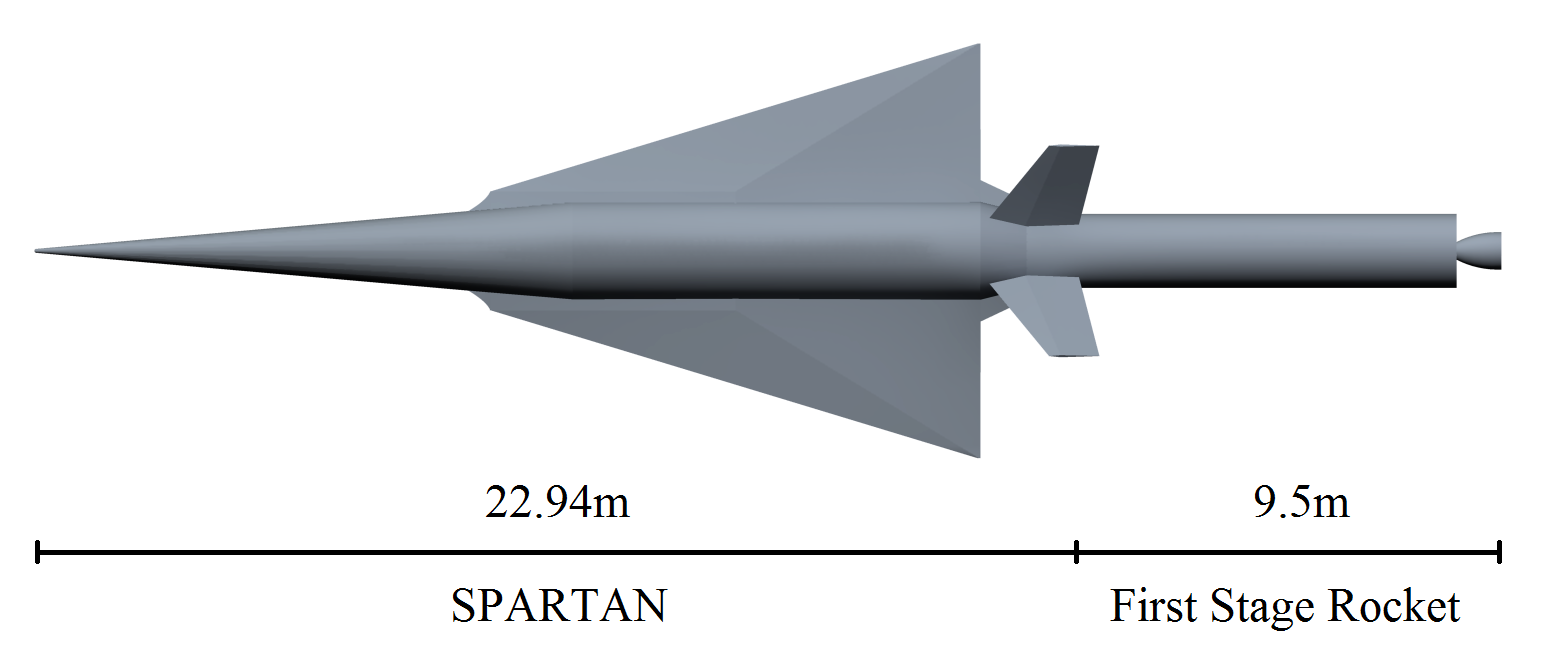
\includegraphics[width=0.7\linewidth]{Figures/NoInternal}
	\caption{The rocket-scramjet-rocket access-to-space system, including the SPARTAN accelerator [CITATION].}
	\label{fig:NoInternal}
\end{figure}
\begin{figure}
	\centering
	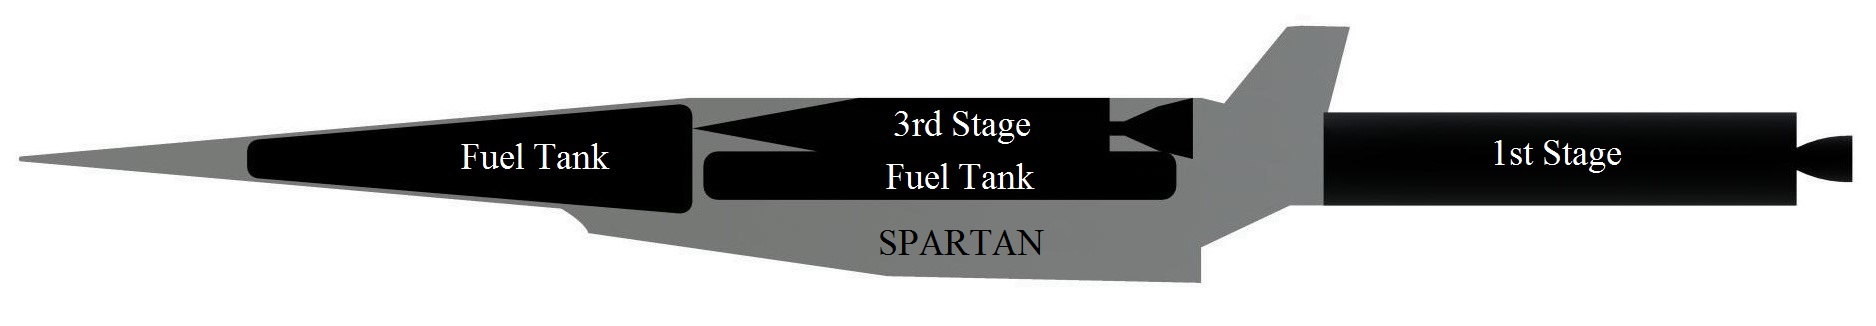
\includegraphics[width=0.7\linewidth]{Figures/INTERNALS}
	\caption{Side view of the rocket-scramjet-rocket system including internals of the SPARTAN vehicle[CITATION].}
	\label{fig:INTERNALS}
\end{figure}
The SPARTAN is a scramjet-powered accelerator designed to operate between approximately Mach 5 and Mach 9. The SPARTAN is accelerated to Mach 5 by a rocket-powered first stage, and at the end of the SPARTAN's acceleration, a rocket-powered third stage is separated which carries a payload to orbit. 
The SPARTAN has a total length of 22.94m, with a wingspan of XXX. The SPARTAN weighs a total of 9819kg, including the third stage, and carries 1562kg of LH2 propellant. The SPARTAN is powered by four underslung C-REST scramjet engines, sized to a capture width of 0.65m.


The use of a scramjet engine improves the specific impulse of the SPARTAN compared to rocket-powered vehicles, and eliminates the necessity for oxidiser to be carried on board. Carrying only fuel on board the vehicle allows the SPARTAN to have a design similar to a traditional aircraft, including avionics and landing gear. The aerodynamic capabilities and avionic systems of the scramjet stage allow it to return to its initial launch site, and land horizontally on a traditional runway. After landing, the vehicle will be checked and re-fuelled, and will then be ready to launch again. The increased reusability that this will afford over similarly sized launch systems will enable the cost-per-kg of launch to be reduced. 

\begin{figure}
\centering
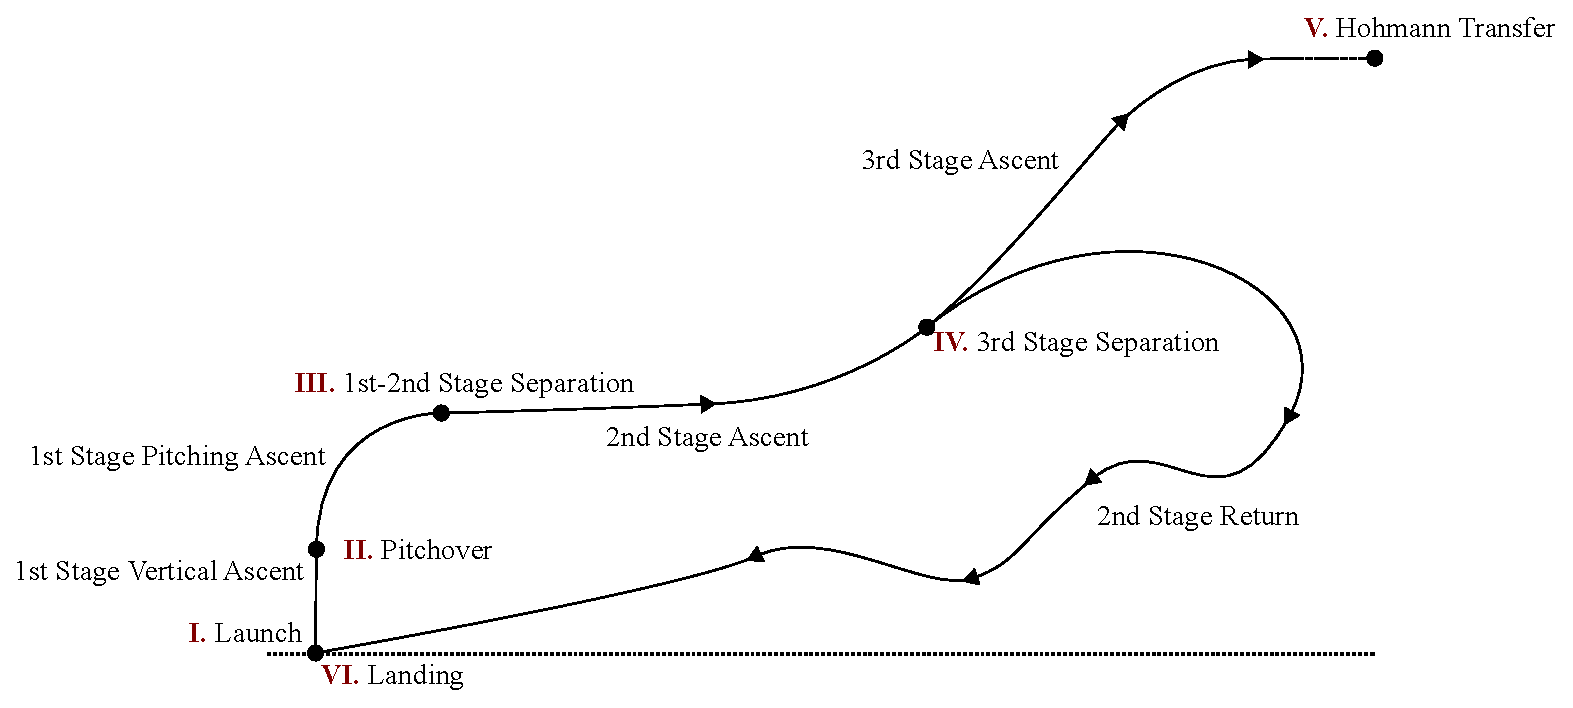
\includegraphics[width=0.9\linewidth]{Figures/Traj}
\caption{A representative view of the trajectory of the rocket-scramjet-rocket launch system incorporating the SPARTAN accelerator.}
\label{fig:Traj}
\end{figure}


The trajectory of the rocket-scramjet-rocket launch system is shown in Figure \ref{fig:Traj}. The system launches vertically under rocket power, and pitches over until close to horizontal flight. The SPARTAN separates from the first stage rocket at Mach 5, the minimum operable Mach number of the scramjet engines. The SPARTAN then accelerates until approximately Mach 9, at which time a pull-up manoeuvre is performed and the third stage rocket is released. The third stage rocket then accelerates, exits the atmosphere, and performs a circularisation burn. At this point a Hohmann transfer is performed to reach the desired orbit. Meanwhile, the SPARTAN turns and flies back to the initial launch site.
The launch ascent profile of the rocket-scramjet-rocket system incorporating the SPARTAN vehicle has been analysed and optimised in previous studies. However, the fly-back of the SPARTAN must be simulated to ensure that the full reusability of the SPARTAN is achievable. This fly-back is crucial to the feasibility of the system, and the amount of fuel necessary to perform the fly-back may have a large effect on the payload-to-orbit of the system. 

It is desirable for the SPARTAN to perform a minimum-fuel fly-back to the initial launch site, with the best-case scenario being for the fly-back to use no fuel at all. However, for a hypersonic trajectory a fully glide-back return flight is most likely unobtainable due to the large initial velocity at the beginning of the fly-back trajectory. 
In previous studies, the maximum separation velocity for glide-back to be feasible has been found to be between Mach 3-4, with higher initial velocities requiring fly-back under power.

Powered fly-back may be achieved either through the use of the existing airbreathing engines, or by using additional engines added for the fly-back only\cite{Mehta2001,Hellman,Wilhite1991}. 
The addition of subsonic engines powering a constant velocity cruise-back phase allows the accelerator to return to base with a similar trajectory to that of a traditional aircraft, allowing the velocity and altitude of the accelerator to be precisely controlled. However, the addition of subsonic engines necessary for cruise-back increases the mass of the vehicle significantly, leading to decreased mass efficiency and increased design complexity\cite{Hellman}. 

The use of the existing hypersonic airbreathing engines during the fly-back allows for range to be added to the return trajectory, without the inclusion of additional engines. The hypersonic airbreathing engines can be throttled on at appropriate times during the fly-back, when they will be most impactful on the return trajectory range. However, the hypersonic airbreathing engines may only be used within their operating region, and vary in thrust and efficiency dependent on flight conditions. The hypersonic airbreathing engines have maximum efficiency at low Mach numbers\cite{Preller2017}. However this must be balanced by the thrust variation with dynamic pressure and inlet conditions, which vary with the trajectory path and angle of attack of the vehicle. This added complexity requires the fly-back trajectory to be optimised to find the most efficient flight path for return to the launch site, and to ensure that the return of the vehicle under its own power is viable. 


Vehicles using high-speed airbreathing propulsion in return flight have been investigated in a study by Tsuchiya and Mori\cite{Tsuchiya2005}.  Tsuchiya and Mori investigate two conceptual launch vehicles; a vehicle powered solely by airbreathing propulsion returning after separation of an orbital stage at Mach 5.1, and an airbreathing/rocket vehicle returning after a separation at Mach 6.8\cite{Tsuchiya2005}. 
These boosters fly to a downrange distance of 600-625km from the launch site, and separate from the orbital accelerator at a dynamic pressure of 15kPa\cite{Tsuchiya2005}. At the start of their respective return trajectories, both boosters turn with a bank angle of 130-145$^\circ$. Both the fully-airbreathing and partially-airbreathing vehicles ignite their airbreathing engines for 'several tens of seconds' at approximately Mach 3.5, in order to extend the flight range of the vehicles and return to the initial launch site\cite{Tsuchiya2005}. Less than 5\% of the vehicles initial propellant was required to return the vehicles to the initial launch sites\cite{Tsuchiya2005}.

When compared to the vehicles investigated by Tsuchiya and Mori\cite{Tsuchiya2005}, the SPARTAN has been shown to separate from its third stage rocket at a considerably higher Mach number of Mach 9.1, as well as at a considerably higher dynamic pressure of 33.9kPa. The SPARTAN must also cover a longer fly-back range of 840km. In addition, the C-REST scramjet engines are limited to operating at hypersonic speeds of Mach 5.1 or higher. These design differences create substantially more challenging conditions than those studied by Tsuchiya and Mori. It is desired to investigate the ability of the SPARTAN to return to the launch site following separation at these conditions. 

The aim of this paper is to find the minimum-fuel fly-back trajectory for the SPARTAN vehicle, from a representative third stage separation location. 







%\subsection{Third Stage}

%The third stage rocket weighs a total of 3300kg, and is powered by a SpaceX LOX-kerosene Kestrel engine, weighing 52kg. The third stage rocket is protected while in-atmosphere by a heat shield weighing 130.9kg. The heat shield is constructed from a phenolic cork cylinder, carbon-carbon nose cone, and tungsten tip. When the third stage reached 10pa the heat shield is discarded, as aerodynamic heating is assumed to be negligible at this point. 
%\begin{figure}
	%\centering
	%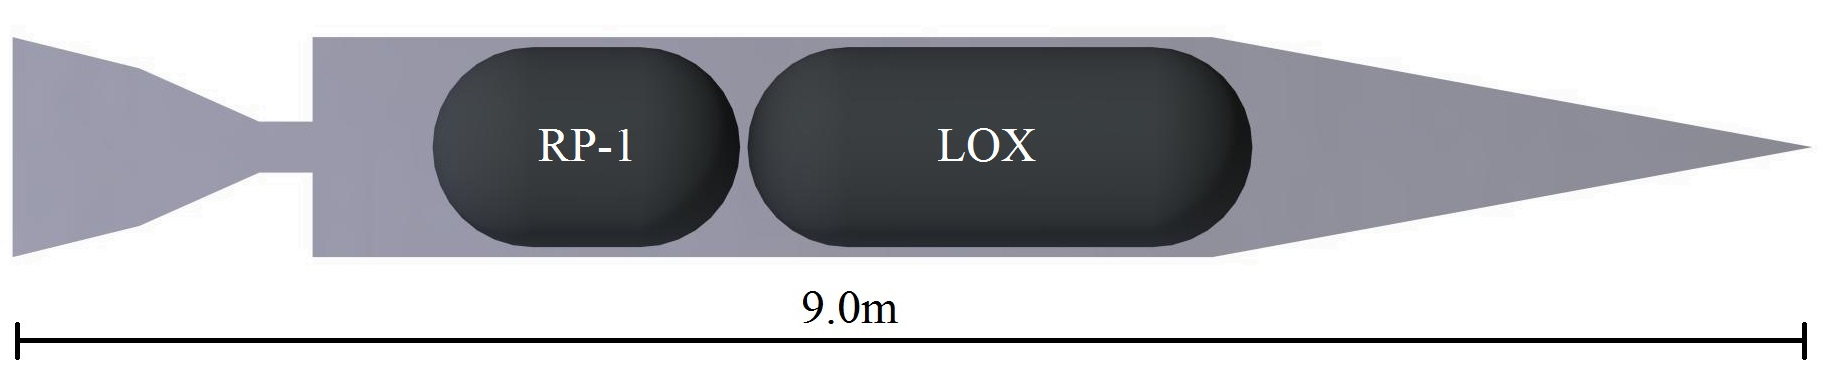
\includegraphics[width=0.7\linewidth]{Figures/3rdStage}
	%\caption{}
	%\label{fig:3rdStage}
%\end{figure}



\section{Aerodynamics}
 This study utilises CART3D to calculate the aerodynamics of the SPARTAN vehicle\cite{CART3D}. CART3D is an inviscid CFD solver for the preliminary design of aerospace vehicles. CART3D utilises adjoint-based mesh refinement with a Cartesian cut-cells approach to produce a mesh refined iteratively to fit a flow solution\cite{Aftosmis1997}. CART3D has been used to generate the aerodynamics of the SPARTAN vehicle due to its applicability over a wide Mach number range, and its robustness across multiple flow solutions. CART3D has previously been used to analyse hypersonic vehicles, and has shown good agreement with experimental data across multiple studies \cite{Sagerman2017,Aftosmis2011}. CART3D has been run for Mach numbers from 0.2 to 9, and for angle of attack values from 0$^\circ$ to 10$^\circ$. An example case is shown in Figure \ref{fig:M7AoA6}, for Mach 7, 6$^\circ$ angle of attack. Figures \ref{fig:Cl} and \ref{fig:Cd} show the lift and drag coefficients of the SPARTAN vehicle over the range of Mach numbers and angle of attack values tested. 
 
 For the purposes of this study, a point mass model is used, and the SPARTAN is assumed to be trimmed at all  conditions during flight.
 
 \begin{figure}
 	\centering
 	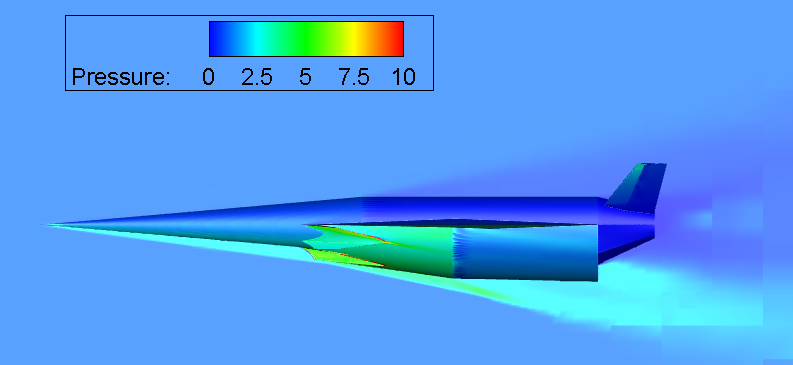
\includegraphics[width=0.7\linewidth]{Figures/M7AoA6}
 	\caption{Normalised pressure contours around the SPARTAN accelerator calculated using CART3D, for Mach 7, 6$^\circ$ angle of attack flight}
 	\label{fig:M7AoA6}
 \end{figure}

\begin{figure}
\centering
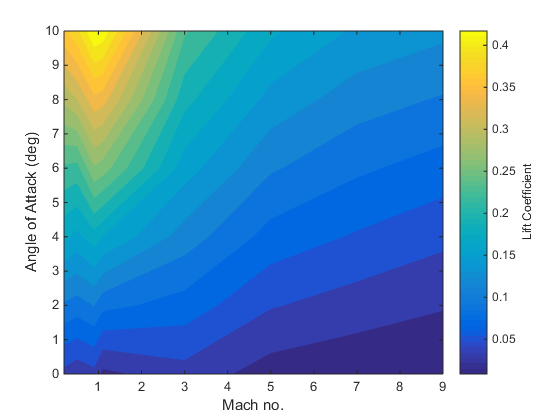
\includegraphics[width=0.6\linewidth]{Figures/Cl}
\caption{Lift coefficient of the SPARTAN accelerator calculated using CART3D, over the flight range of Mach number and angle of attack values. $A_{ref} = 62.77m^2$.}
\label{fig:Cl}
\end{figure}
\begin{figure}
\centering
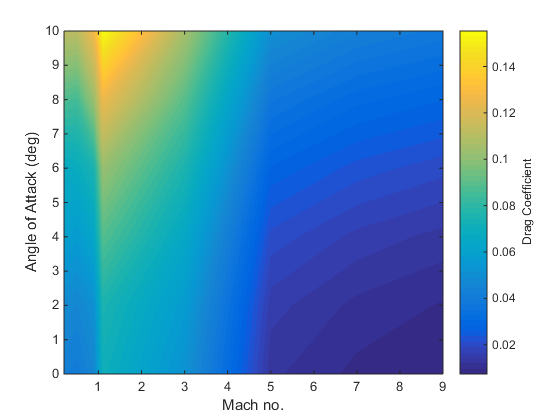
\includegraphics[width=0.6\linewidth]{Figures/Cd}
\caption{Drag coefficient of the SPARTAN accelerator calculated using CART3D, over the flight range of Mach number and angle of attack values. $A_{ref} = 62.77m^2$.}
\label{fig:Cd}
\end{figure}



\section{Trajectory Optimisation}
The optimisation of the trajectories in this study are performed using LODESTAR. LODESTAR is a trajectory optimisation tool under development at The University of Queensland for hypersonic vehicle analysis. LODESTAR generates optimal trajectories given a target cost function, and sets of initial and end constraints. LODESTAR utilises the pseudospectral method optimisation software GPOPS-2\cite{Patterson2015}. 

The pseudospectral method is a form of direct spectral collocation, in which a spectral collocation method is used to approximate the optimal control problem as a nonlinear programming problem. The pseudospectral method offers an accurate, robust optimal control solution with relatively good computational times, making it particularly applicable to complex hypersonic vehicle trajectories.  The pseudospectral method has been successfully applied in a variety of aerospace applications, and GPOPS-2 is used widely within the aerospace field as a solver for complex aerospace vehicle trajectories.


\subsection{Dynamic Model}

The SPARTAN is simulated in a geodetic rotational reference frame \cite{Josselyn2002a}: 

\begin{equation}
\dot{r} = v \, \sin \gamma
\end{equation}

\begin{equation}
\dot{\xi} = \frac{v \, \cos \gamma \, \cos \zeta}{r \, \cos \phi}
\end{equation}

\begin{equation}
\dot{\phi} = \frac{v\,\cos\gamma\,\sin\zeta}{r}
\end{equation}
\begin{equation}
\dot{\gamma} = \frac{T\,\sin\alpha}{m\,v}+ (\frac{v}{r}-\frac{\mu_E}{r^2 \,v})\,\cos\gamma + \frac{L}{m\,v}
+ \cos\phi[2\,\omega_E\, \cos\zeta + \frac{\omega_E^2\, r}{v}(\cos\phi\,\cos\gamma+\sin\phi\,\sin\gamma\,\sin\zeta)]
\end{equation}
\begin{equation}
\dot{v} = \frac{T\,\cos\alpha}{m}-\frac{\mu_E}{r^2}\,\sin\gamma - \frac{D}{m}
+ \omega_E^2 r\,\cos\phi(\cos\phi\,\sin\gamma-\sin\phi\,\cos\gamma\,\sin\zeta)
\end{equation}
\begin{equation}
\dot{\zeta} = -\frac{v}{r}\tan\phi\,\cos\gamma\,\cos\zeta +2\,\omega_E\,\cos\phi\,\tan\gamma\,\sin\zeta - \frac{\omega_E^2 r}{v\,\cos\gamma}\,\sin\phi \, \cos\phi\,\cos\zeta-2\omega_E\,\sin\phi 
\end{equation}

Where $r$ is the radius from the centre of Earth, $\xi$ is longitude, $\phi$ is latitude, $\gamma$ is flight path angle,$v$ is velocity and $\zeta$ is heading angle. The drag and lift of the SPARTAN are calculated using the standard aerodynamic coefficients;

\begin{equation}
F_d = \frac{1}{2} \, \rho \, C_D \, v^2 \, A ,
\end{equation}
\begin{equation}
F_L = \frac{1}{2} \, \rho \, C_L \, v^2 \, A .
\end{equation}

\section{Flyback Trajectory Analysis}
The flyback of the SPARTAN is optimised using LODESTAR. The flyback is optimised for minimum fuel flyback, with initial conditions constrained to be similar to the intended third stage release point, and end position constrained within XXXrad of the initial launch site, at XX,XX. The angle of attack is limited to 10$^\circ$, to ensure vehicle stability. The bank angle is limited to 90$^\circ$. The dynamic pressure is limited to 50kPa, the structural limit of the vehicle. The scramjet engines are limited to only operate above 20kPa dynamic pressure.
The end of the trajectory is constrained to under XXXm altitude, and greater than XXXdeg trajectory angle. The end velocity is left unconstrained. It is assumed that for an optimal flyback trajectory, the end velocity will be minimised. 
It is assumed that the vehicle is able to carry any necessary fuel is addition to the fuel required during the ascent trajectory. 

\subsection{Optimised Trajectory}

The optimised fly-back trajectory is shown in Figures \ref{fig:Traj1}, \ref{fig:Traj2}, \ref{fig:Traj3} and \ref{fig:lon-lat}. The potential Isp is shown along the trajectory, this is the Isp obtainable from the C-REST engines should they be throttled on. This fly-back is initiated from 2.53 rad longitude, -0.135 rad latitude, 34.5km altitude, 2.9$^\circ$ trajectory angle, 2881m/s velocity and 102$^\circ$ heading angle. These conditions correspond to the conditions of optimal third stage release. 

\begin{figure}
	\centering
	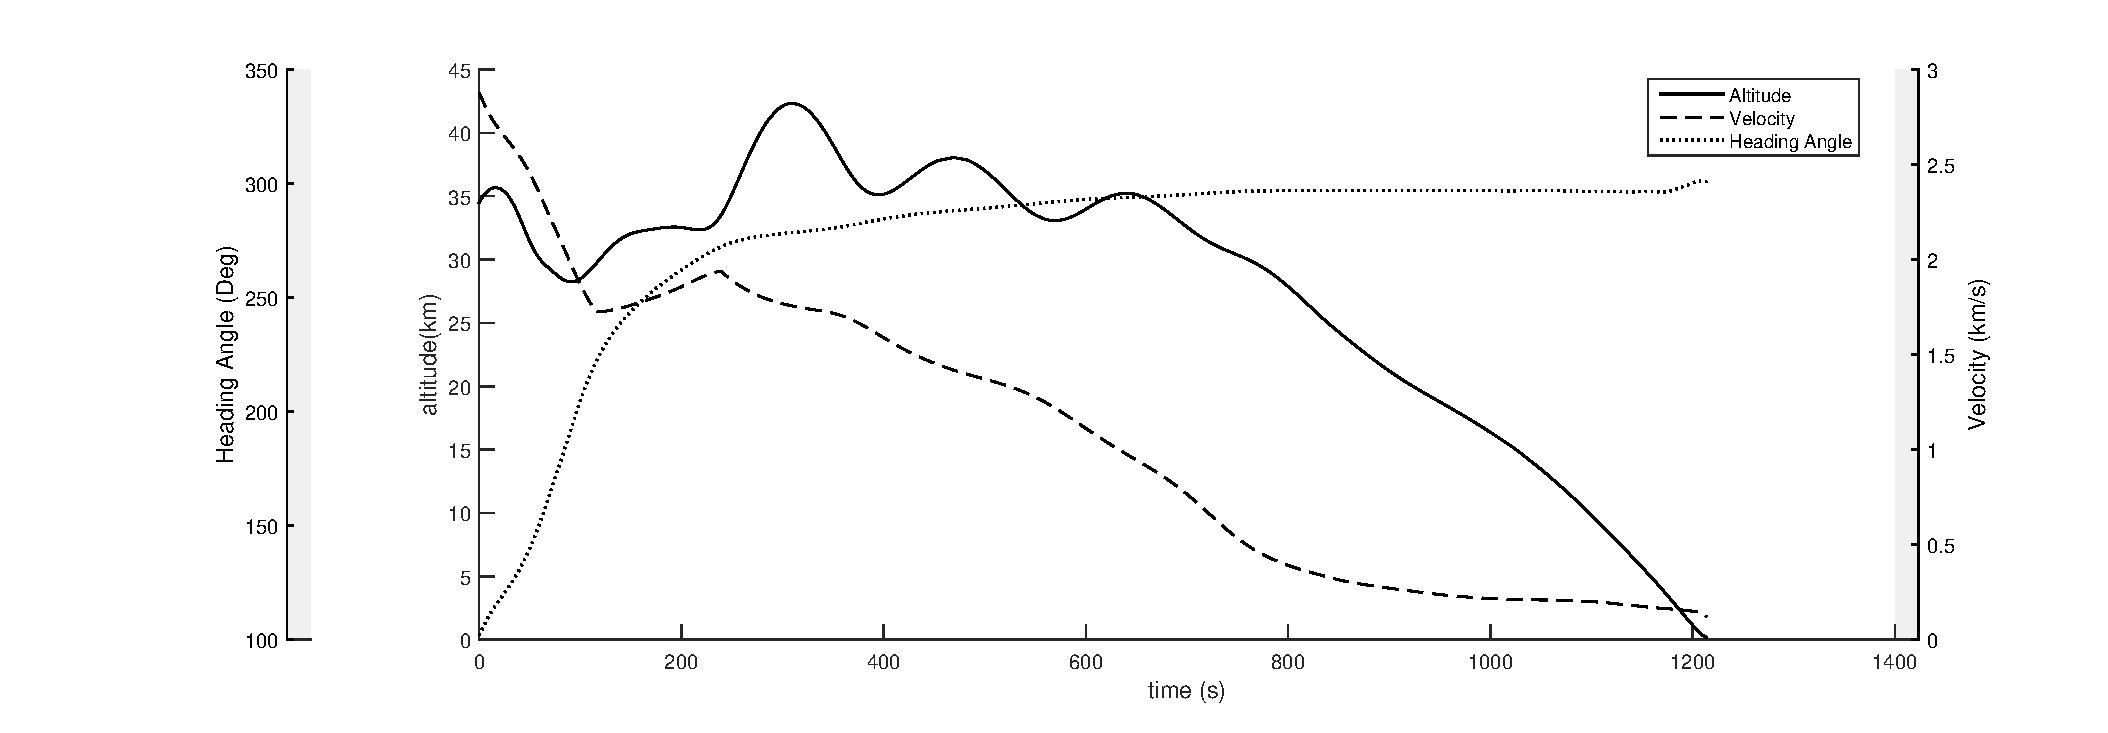
\includegraphics[width=0.9\linewidth]{Figures/Traj1}
	\caption{Trajectory data for the fly-back of the SPARTAN vehicle. Optimised for minimum fuel using LODESTAR.}
	\label{fig:Traj1}
\end{figure}
\begin{figure}
	\centering
	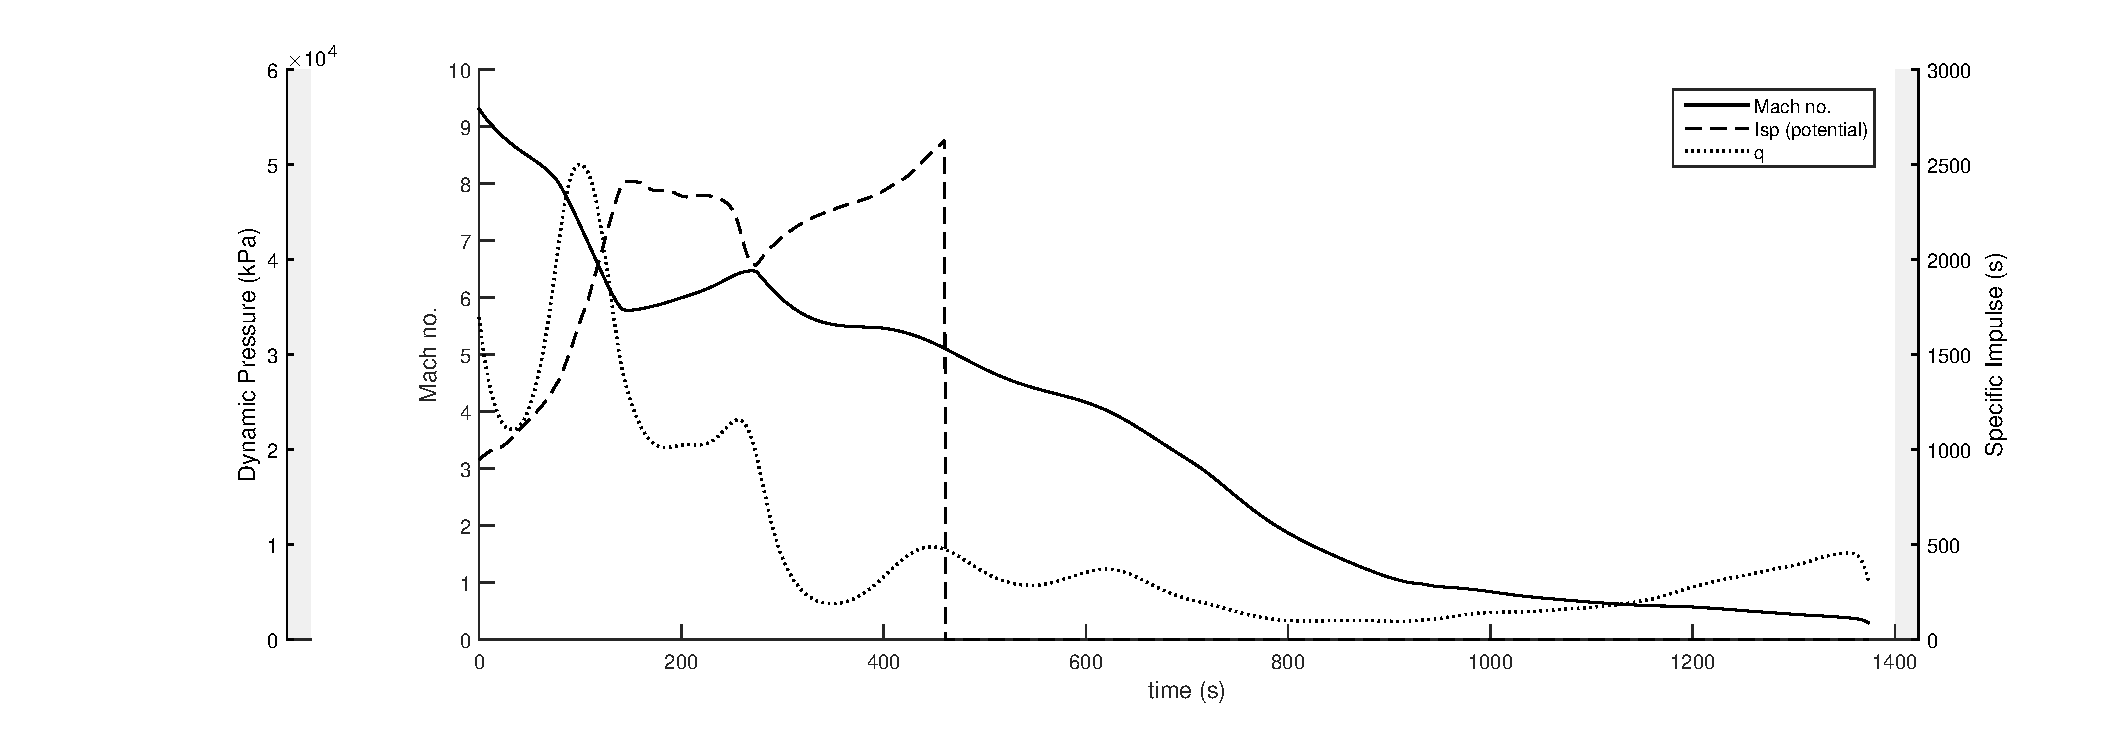
\includegraphics[width=0.9\linewidth]{Figures/Traj2}
	\caption{Aerodynamic and performance data for the optimised fly-back of the SPARTAN vehicle.}
	\label{fig:Traj2}
\end{figure}
\begin{figure}
	\centering
	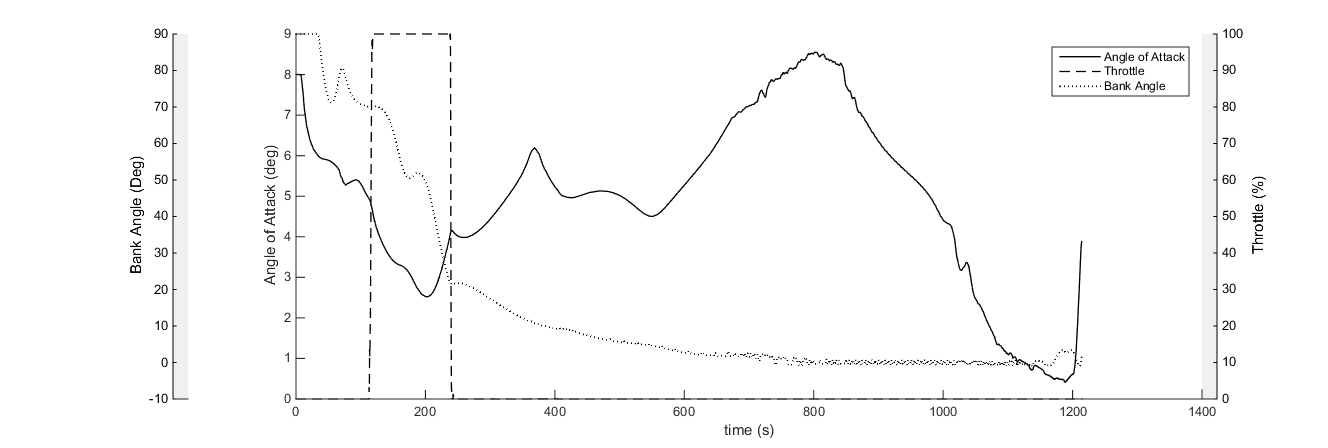
\includegraphics[width=0.9\linewidth]{Figures/Traj3}
	\caption{Control data for the optimised fly-back of the SPARTAN vehicle.}
	\label{fig:Traj3}
\end{figure}

\begin{figure}
	\centering
	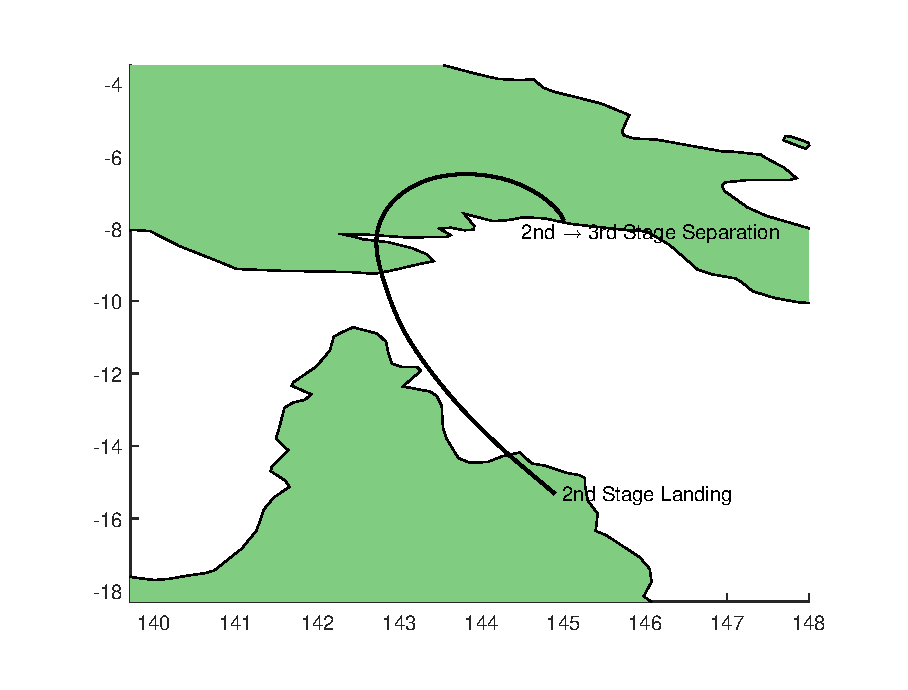
\includegraphics[width=0.5\linewidth]{Figures/lon-lat}
	\caption{Ground track of the optimised fly-back of the SPARTAN vehicle.}
	\label{fig:lon-lat}
\end{figure}

The SPARTAN starts at the maximum bank angle of 90$^\circ$, and sustains this bank angle for 34.4s. At this point, the altitude of the SPARTAN has decreased, and the vehicle is close to hitting the dynamic pressure of 50kPa. To avoid exceeding this limit, the bank angle is reduced to 71.2$^\circ$, allowing the vehicle to generate sufficient lift to slow its descent. The bank angle in then increased again, to 80.7$^\circ$ at 70.8s. After this time, the bank angle is reduced gradually, reaching 10$^\circ$ at 384.4s, at which time the heading angle has reached 283.1$^\circ$. Soon after the bank angle has begun to reduce, at 118.7s flight time and Mach 5.71, the scramjet engines are throttled on. The SPARTAN burns for 119.8s, using a total of 166.0kg of fuel. The SPARTAN engines are throttled on at a point of high potential specific impulse, at a low Mach number. The point of engine ignition is limited by the lower dynamic pressure limit of 20kPa, which is nearly reached during burn. The angle of attack of the vehicle is controlled during the burn in order to maximise the specific impulse of the scramjet engines. The SPARTAN performs several 'skips' after the scramjet burn.
 At the end of the trajectory the SPARTAN pulls up, and reaches 200m altitude at -9.6$^\circ$ trajectory angle and 119.8m/s velocity. After this point it is assumed that the SPARTAN is able to perform a landing on a standard runway. 

The optimised fly-back increases the fuel usage of the SPARTAN by 10.6\%. This study assumes that the extra fuel necessary for the fly-back is able to be incorporated within the SPARTAN. However, realistically the additional fuel necessary for the fly-back will reduce the amount of fuel able to be used during the scramjet acceleration, and consequently reduce the velocity at third stage separation.

\section{Sensitivity Analysis}
To investigate the sensitivity of the fly-back to the vehicle design; the aerodynamic parameters and thrust efficiency of the SPARTAN are modified, and optimised trajectories calculated. The drag coefficient is varied by $\pm 5\%$. 

\section{Conclusion}
The fly-back trajectory of the SPARTAN hypersonic vehicle has been investigated, from separation at 7.7$^\circ$S,145.0$^\circ$E to landing at 15.3$^\circ$S,144.9$^\circ$E. The aerodynamics of the SPARTAN are calculated using CART3D, and inviscid CFD package, over the range of Mach numbers and angle of attack values of flight. The optimal trajectory of the SPARTAN has been found to fly-back to the initial launch position with minimum fuel. The optimal trajectory has been found by calculating the trajectory using the optimal control program LODESTAR. It has been found that the SPARTAN is capable of returning to its initial launch position, using 166.0kg of fuel. The SPARTAN lands at 95.4m/s.  

This study indicates that the fly-back of a hypersonic launch vehicle which separates at a Mach number greater than nine and then returns to its initial launch site is feasible. 

\section*{Acknowledgments}


\bibliography{library}

\end{document}
